\chapter{Experiments And Observations}
\label{ch:experiments-and-observations}

\section{Initial Pheromone Concentration Sensibility}

Due to the model of node selection agents are sensitive to the initial pheromone concentration presented by the environment around them. This happens because the probability of choosing a neighbour node swings form $0$ to a $100$ percent very swiftly, causing the agents to get trapped.

This experiment investigates how different initial pheromone concentrations in the environment and the amount of pheromone each agent is capable of depositing in each interaction affect the agents navigation through the space. It has objective to determine what values of these two parameters are acceptable to use in the other experiments.

Firstly, let's examine the case when all the nodes of the environment are created with no initial concentration of \emph{Forage} pheromone (Figure \ref{fig:initial-a}). When the agent is deciding which node it is going to make the first move to, all neighbours have the same probability of being picked, because of the $0$ of pheromone concentration (Figure \ref{fig:initial-b}). So as it was programmed to, the agent picks one node at random. But before moving to the next node it lays a bit of pheromone, suppose the concentration deposited is $0.1$. When the move is done, the environment around the agent should look like the one pictured in Figure \ref{fig:initial-c}.

\begin{figure}[H]
\myfloatalign
\subfloat[Initial environment]
{\label{fig:initial-a}
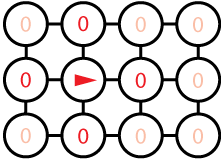
\includegraphics[width=.3\linewidth]{gfx/initial-01}} \quad
\subfloat[Initial probabilities]
{\label{fig:initial-b}
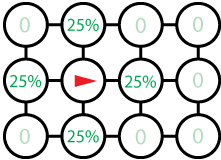
\includegraphics[width=.3\linewidth]{gfx/initial-02}} \\
\subfloat[Environment after move 1]
{\label{fig:initial-c}
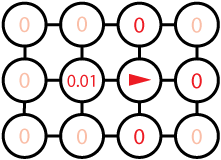
\includegraphics[width=.3\linewidth]{gfx/initial-03}} \quad
\subfloat[Probabilities after move 1]
{\label{fig:initial-d}
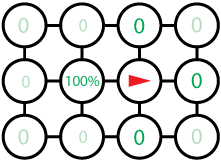
\includegraphics[width=.3\linewidth]{gfx/initial-04}} \\
\subfloat[Environment after move 2]
{\label{fig:initial-e}
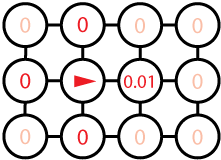
\includegraphics[width=.3\linewidth]{gfx/initial-05}} \quad
\subfloat[Probabilities after move 2]
{\label{fig:initial-f}
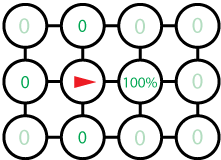
\includegraphics[width=.3\linewidth]{gfx/initial-06}}

\caption{Affect of initial pheromone concentration at zero}\label{fig:initial}
\end{figure}

Now it is time for the agent to move again. Firstly the agent reads the pheromone intensity in each of the neighbour nodes, after it computes where it is more likely to move. For all the nodes around the agent apart from the one it has just moved from have $0$ pheromone intensity in them, the agent is certain to move back to the previous node (Figure \ref{fig:initial-d}). Before completing the move, it lays pheromone in the current node. When the agent is back to the node it first started from, the scenario repeats and it becomes a cycle. The agent go back and forth, trapped in these two nodes forever, with no changes to explore the environment further. 

It is clear that the environment cannot be initialised with no \emph{Forage} pheromone in its nodes. The question that arises from this is: Is there any pair of values for these two parameters that will allow the agents to navigate in an acceptable fashion?

To answer this question, the experiment was setup with the following configuration:

\begin{table}[H]
\myfloatalign
\begin{tabularx}{\textwidth}{Xll} \toprule
\tableheadline{Property} & \tableheadline{Value} \\ \midrule
Number of lines & 500 \\
Number of columns & 500 \\
Total number of nodes &  250,000 \\
\midrule
Duration of each simulation & 10 s \\
Number of agents & 50 \\
Agent Type & WorkerType \\
Task executed & ForageTask \\
Agent sleep time & 5 ms \\
\bottomrule
\end{tabularx}
\caption{Experiment setup for investigation of initial pheromone concentration}  
\label{tab:setup-1}
\end{table}

In Table \ref{tab:setup-1} the property \emph{Agent sleep time} means how long the agent waits after a task is executed to choose another task to run. This is necessary to slow down agents (in this case the threads that are running the agent), otherwise they would cover the entire space in this 10 seconds only by the fact that they can do it very fast not because they are actively foraging.

The initial pheromone concentration and the amount of pheromone deposited in each interaction by the agents were varied from $0.001$ to $0.04$ in $5$ steps. Each of the possible pair of values for the two parameters has been simulated:

\begin{table}[H]
\myfloatalign
\begin{tabularx}{\textwidth}{XXXXX} \toprule
\tableheadline{1} & \tableheadline{2} & \tableheadline{3} & \tableheadline{4} & \tableheadline{5} \\ \midrule
0.001, 0.001 & 0.001, 0.005 & 0.001, 0.01 & 0.001, 0.02 & 0.001, 0.04 \\
0.005, 0.001 & 0.005, 0.005 & 0.005, 0.01 & 0.005, 0.02 & 0.005, 0.04 \\
0.01, 0.001 & 0.01, 0.005 & 0.01, 0.01 & 0.01, 0.02 & 0.01, 0.04 \\
0.02, 0.001 & 0.02, 0.005 & 0.02, 0.01 & 0.02, 0.02 & 0.02, 0.04 \\
0.04, 0.001 & 0.04, 0.005 & 0.04, 0.01 & 0.04, 0.02 & 0.04, 0.04 \\
\bottomrule
\end{tabularx}
\caption{Variations for initial concentration and amount of pheromone deposited by agents}  
\label{tab:setup-2}
\end{table}

In each case, the colony containing $50$ agents is created at the north of the environment, horizontally centred. The agents execute the \emph{ForageTask} since their creation, they do not analyse any contextual parameters such as other agents, they only try to move through the space using the rules defined by the task.

In order to compare how each possible value pairs in Table \ref{tab:setup-2} affect the resulting navigation of the agents, two samples of  the pheromone trail left by the agents are analysed. The first one is from close to the nest that will enable us to check how is the agents' response to the initial pheromone concentration shortly they have left the nest. The second sample is taken further ahead in the environment, far from the nest. This sample is a good way to test how the agents' own deposit of pheromone will affect the system behaviour, Figure \ref{fig:initial-sample} illustrates how and where the samples are made.

\begin{figure}[H]
  \centering
  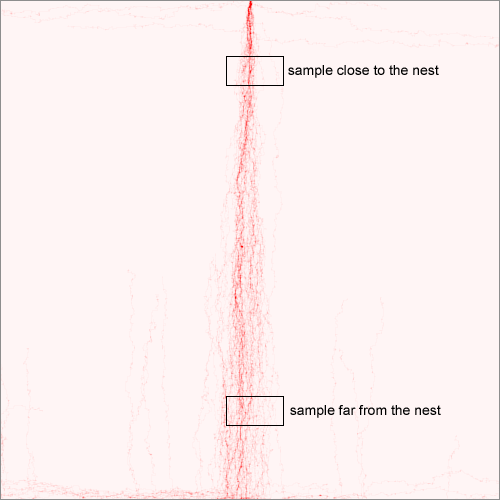
\includegraphics[width=0.5\linewidth]{gfx/initial-sample.png}
  \caption{How the two samples of the environment is made}
  \label{fig:initial-sample}
\end{figure}

Figures \ref{fig:initial-var-close} and \ref{fig:initial-var-far} show the resulting sampling for all possible combination for the initial pheromone concentration and the amount of pheromone deposited by each agent in each interaction.

\begin{figure}[H]
  \centering
  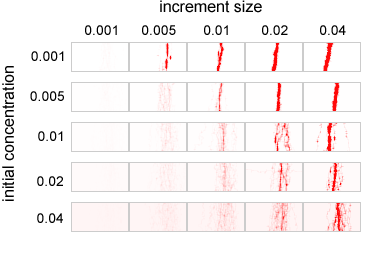
\includegraphics[width=0.6\linewidth]{gfx/initial-variations-close.png}
  \caption{Resulting pheromone trail close to the nest}
  \label{fig:initial-var-close}
\end{figure}


\begin{figure}[H]
  \centering
  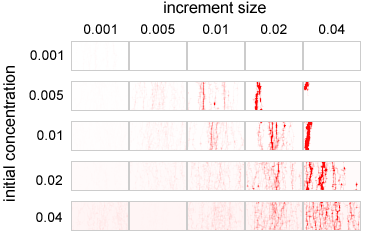
\includegraphics[width=0.6\linewidth]{gfx/initial-variations-far.png}
  \caption{Resulting pheromone trail far from the nest}
  \label{fig:initial-var-far}
\end{figure}

The trails left by the colonies can be compared in relation on how strong they are, how the agents are able to 'scape' them to explore the environment and how it shaped when agents get further from the nest.

Starting from $0.001$ as the amount of pheromone to be deposited by agents in each interaction. It is possible to observe from the figures that two very contrasting behaviours emerge, firstly because the environment has so little pheromone and the update is so small, they weight assigned to each of the neighbour nodes count considerably more than the pheromone deposited by the agents, so the agents end up very dispersed, thus no chemical trail is formed at all. This phenomena is actually seen in many other combination of the parameters, all the cases when the update is $0.001$ in fact. 

When the amount of pheromone deposited by the agents is increased the behaviour of the colony could not be more different than what was seen previously. The agents switch from exploring a large area to be 'trapped' into the pheromone trail. This impedes the agents of exploring the space, what is not desirable for any colony. This behaviour is also seen in other values for the parameters. What seems to be the rule is that if the update is considerable larger than the concentration of pheromone in the environment the agents will start to create a 'bubble' of high pheromone concentration and as consequence they are very unlikely to move to any node outside this area.

It rises the question, why does it happen? The answer is similar to one of the problem in initialising the environment with no pheromone at all. In this case, the critical point is the rate between the initial concentration and the amount deposited by the agents in each interaction.

\begin{figure}[H]
\myfloatalign
\subfloat[]
{\label{fig:update-a}
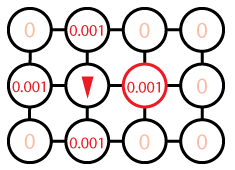
\includegraphics[width=.2\linewidth]{gfx/update-01}} \quad
\subfloat[]
{\label{fig:update-b}
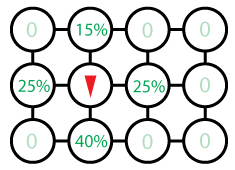
\includegraphics[width=.2\linewidth]{gfx/update-02}} \\
\subfloat[]
{\label{fig:update-c}
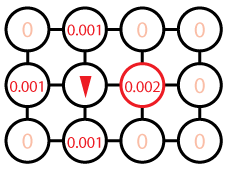
\includegraphics[width=.2\linewidth]{gfx/update-03}} \quad
\subfloat[]
{\label{fig:update-d}
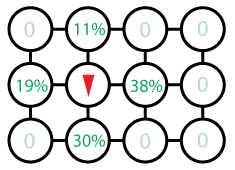
\includegraphics[width=.2\linewidth]{gfx/update-04}} \\
\subfloat[]
{\label{fig:update-e}
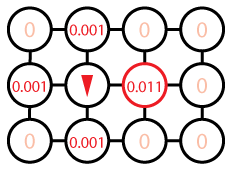
\includegraphics[width=.2\linewidth]{gfx/update-05}} \quad
\subfloat[]
{\label{fig:update-f}
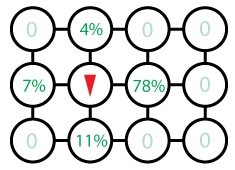
\includegraphics[width=.2\linewidth]{gfx/update-06}}

\caption{Shift of probability depending on agent update}\label{fig:update}
\end{figure}

Figure \ref{fig:update} illustrates how swiftly the probabilities can change depending on the amount of pheromone deposited in the node by agents. The node in red in the picture represents a node that has been updated previously by another agent. In the first scenario (Figure \ref{fig:update-c}) the update was $0.001$, in the second (Figure \ref{fig:update-e}) the pheromone deposited was $0.01$. The probability of the node in red being picked up to be the next node the agent will move to more than doubled. (Figure \ref{fig:update-d} and Figure \ref{fig:update-f}).

Further investigation revealed that the probability of selection increases in a logarithmic-like curve. Figure \ref{fig:prob-inc} shows how the increase in probability progress when the amount of pheromone deposited by the agents increases by multiples of the initial concentration in the environment.

\begin{figure}[H]
  \centering
  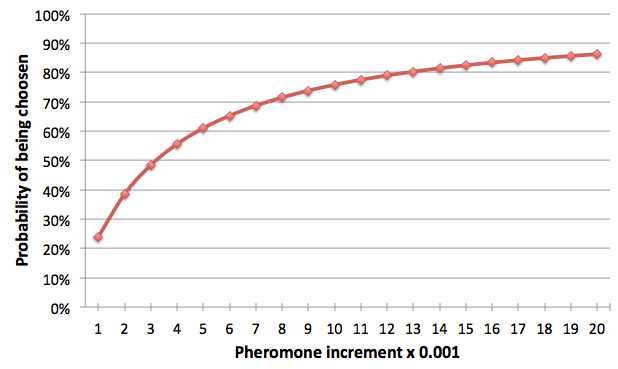
\includegraphics[width=0.6\linewidth]{gfx/probability-increase.png}
  \caption{Increase of probability selection according to the increase of the deposit increment}
  \label{fig:prob-inc}
\end{figure}

It is very tempting to conclude that if the right ratio between the initial pheromone concentration and the increment step used by the agents is found the, problems of the lack of trail formation and the agent confinement in the trail will be solved. However from figures \ref{fig:initial-var-close} and \ref{fig:initial-var-far} it is observed that the same ratio initial concentration/increase step present different results for different values. That is counter intuitive at first, but what actually gives rise to the conditions to create the trails 

but what seems to be necessary condition to form the pheromone trails intense enough to guide the agents, but at the same time not restricting agents to explore the environeent 

Explain that the agents are sensitive to initial pheromone concentration due to the model of node selection.

This experiment is proposed to investigate what parameters are the best to be used in the other experiments.

Explain that there are two variables important here, the initial concentration of pheromone throughout the environment and the amount of pheromone deposited by the agents each time they visit a node.

Explain the how the agents choose to move from one node to another, and why the environment pheromone concentration cannot be initialised with 0.

Tell that the initial concentrations values tried were: 0.001, 0.005, 0.01, 0.02, 0.04. And that each agent could deposit 0.01 of chemical communication pheromone when visiting a node.

Each simulation was run for 10 seconds, each agent resting a minimum of 5 milliseconds in each node.

[add a compiled image with pheromone trail for each variation]

0.001 - the agents get trapped in the pheromone trail that they have deposited and end up not being able to explore the environment.

0.005 - Much better result, the agents are able to explore the environment in a way they could not before. But it is quite unlikely for agents to 'break' from the pheromone trail and explore new areas.

0.01 - Most of the agents are able to follow the main pheromone trail, which with time get reinforced by the agent's themselves. But at the same time the agents are able to 'break' from the main pheromone trail and explore new parts of the space available form them.

0.02 - Agents still have a main pheromone trail but they tend to disperse quite a lot over time.

0.04 - No main pheromone trail present at all. The agents get too much dispersed, impossible to communicate properly, for instance when foraging food.

Explain that for the reasons above all the other experiments are run using 0.01 as the initial pheromone concentration. In fact it was observed that what is important is that the initial concentration has to match the agent's capacity of pheromone deposition. So other initial pheromone concentrations could be used, as long as the amount of pheromone deposited by each agent would have been changed to match the initial concentration.

\section{Warning Pheromone Response}
\label{sec:warn-phero-inv}
In this experiment the response of the agents to a warning communication stimulus is tested.

Describe the experiment setup.

Explain that the experiment is done in two phases, the first one the agents react only to amount of warning pheromone and the second one the agents react also to the number of other agents they meet that are traveling in the opposite direction and are not caring food.

Add block diagrams that explain the algorithms the agents use to decide on task selection.

Discuss the results. [experiment not done yet]
Results should vary with the use of different parameters, such as the number of agents traveling in the opposite direction before the agent abort the current task and change to findNestAndHide task.

\section{Forage Radius Investigation}
\label{sec:forage-radius-inv}

In this experiment the radius of action of the forage pheromone is varied in order to check the effects in the amount of food the colony is capable of forage.

Explain how the variation of the radius actually impact the pheromone deposition. Add images to explain how the pheromone is actually deposited depending on the radius. Explain that the deposition follow 1/x.

Describe the experiment setup

Radius values used in the experiment were 0, 1 and 2.

Add simulation images.

Add the simulation data results

Discussion: Agents depend on the pheromone trail that they create to forage food, when the radius is 0 the agents are able to forage well, because the trail is well defined, but this indirectly limit the amount of agents recruited as the width of the main pheromone trail is very narrow. 

Using radius equals to one the main pheromone trail gets wider allowing more agents to be pointed to the right direction.

Now when using radius equals to two, the pheromone trail gets too wide, this gets on the way of the agents as they do not have a clear direction to follow when they are within the trail. 

Add image of an agent history, showing how much steps it spend inside the trail going up and down, going nowhere.